\documentclass[aspectratio=169,10pt]{beamer}

% ── Tema ──────────────────────────────────────────────────────────
\usetheme{Madrid}
\usecolortheme{default}
\setbeamertemplate{frame numbering}[fraction]
\setbeamercolor{background canvas}{bg=white}

% ── Paquetes ──────────────────────────────────────────────────────
\usepackage[utf8]{inputenc}
\usepackage[T1]{fontenc}
\usepackage{booktabs}
\usepackage{multicol}
\usepackage{tikz}
\usetikzlibrary{arrows.meta, positioning, shapes, fit}
\usepackage{graphicx}
\usepackage{amsmath, amssymb}
\usepackage{caption}

% ── Macros ────────────────────────────────────────────────────────
\definecolor{azul}{HTML}{1a5092}
\definecolor{rojo}{HTML}{b22222}
\definecolor{verde}{HTML}{27ae60}
\definecolor{gris}{HTML}{7f8c8d}
\setbeamercolor{titlelike}{fg=azul}
\setbeamercolor{structure}{fg=azul}
\setbeamercolor{alerted text}{fg=rojo}
\setbeamercolor{palette primary}{fg=white, bg=azul}
\setbeamercolor{palette secondary}{fg=white, bg=azul!80}
\setbeamercolor{palette tertiary}{fg=white, bg=azul!60}

\newcommand{\pct}[1]{\textbf{#1\%}}
\newcommand{\cmark}{\textcolor{verde}{$\cmark$}}
\newcommand{\xmark}{\textcolor{rojo}{$\times$}}
\newcommand{\code}[1]{\texttt{#1}}

% ── Documento ─────────────────────────────────────────────────────
\begin{document}

% ══════════════════════════════════════════════════════════════════
\begin{frame}[plain]
  \centering
  \vfill
  {\Huge\bfseries\color{azul} predWC}\\[0.3cm]
  {\Large World Cup 2026 --- Knockout Predictor}\\[1cm]
  {\small Modelo stacking para predicci\'on de resultados\\[0.2cm]
   en fase eliminatoria del Mundial 2026}\\[1.5cm]
  {\footnotesize \today}
  \vfill
\end{frame}

% ══════════════════════════════════════════════════════════════════
\begin{frame}{Motivaci\'on y problema}
  \textbf{Problema:} predecir el ganador de cada partido eliminatorio
  del Mundial 2026 (48 selecciones, 3 rondas KO).\\[0.4cm]

  \textbf{Desaf\'ios:}
  \begin{itemize}
    \item Datos limitados: solo partidos previos entre selecciones
    \item Desbalance de clases: empates son menos frecuentes (\~{}23\%)
    \item Sin leakage temporal: no usar informaci\'on futura
    \item Scores exactos necesarios para visualizaci\'on
  \end{itemize}
  \vspace{0.3cm}
  \textbf{Soluci\'on:} stacking ensemble + Dixon-Coles,
  entrenado con split temporal 80/20 sobre 8\,204 partidos (2018--2026).
\end{frame}

% ══════════════════════════════════════════════════════════════════
\begin{frame}{Pipeline de datos}
  \centering
  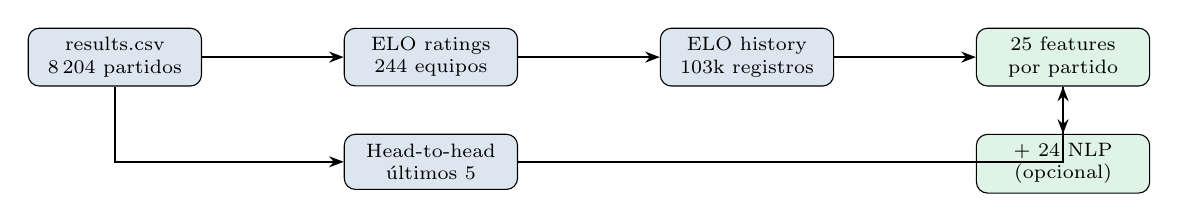
\begin{tikzpicture}[
      node distance=0.6cm and 1.8cm,
      box/.style={draw, rounded corners, minimum width=2.2cm,
                  minimum height=0.7cm, align=center, font=\scriptsize},
      arrow/.style={-{Stealth[scale=0.8]}, thick} ]
    \node[box, fill=azul!15] (results)   {results.csv\\ 8\,204 partidos};
    \node[box, fill=azul!15, right=of results] (elo)     {ELO ratings\\ 244 equipos};
    \node[box, fill=azul!15, right=of elo] (elohist) {ELO history\\ 103k registros};
    \node[box, fill=azul!15, below=of elo] (h2h)    {Head-to-head\\ \'ultimos 5};
    \node[box, fill=verde!15, right=of elohist] (features) {25 features\\ por partido};
    \node[box, fill=verde!15, below=of features] (nlp) {+ 24 NLP\\ (opcional)};

    \draw[arrow] (results) -- (elo);
    \draw[arrow] (elo)     -- (elohist);
    \draw[arrow] (results.south) |- (h2h);
    \draw[arrow] (elohist)  -- (features);
    \draw[arrow] (h2h)     -| (features);
    \draw[arrow] (features) -- (nlp);
  \end{tikzpicture}
  \vspace{0.3cm}

  \begin{itemize}
    \item Fuente: \texttt{github.com/martj42/international\_results}
    \item ELO est\'atico + historial desde \texttt{eloratings.net}
    \item NLP opcional: noticias + YouTube sentiment
  \end{itemize}
\end{frame}

% ══════════════════════════════════════════════════════════════════
\begin{frame}{Ingenier\'ia de caracter\'isticas (25 features)}
  \begin{multicols}{2}
    \textbf{Equipo local (8):}
    \begin{itemize}\small
      \[]{\footnotesize Partidos jugados (rolling)}
      \item Promedio goles a favor / en contra
      \item Diferencia de goles media
      \item \% victorias, empates, derrotas
      \item Forma reciente (\'ultimos 5)
    \end{itemize}

    \textbf{Equipo visitante (8):} {\small mismas 8 m\'etricas}
  \end{multicols}

  \textbf{ELO y derivadas (4):}
  \[
  \text{ELO local},\quad \text{ELO visitante},\quad
  \Delta\text{ELO},\quad \Delta\text{goal diff}
  \]

  \textbf{Contexto (5):}
  victorias/empates H2H, peso del torneo, local\'ia\\[0.2cm]

  \textbf{Ponderaci\'on temporal:}
  \begin{itemize}\small
    \item Ventana: \'ultimos 10 partidos
    \item Decaimiento exponencial: \emph{half-life} 180 d\'ias
    \item Peso por ELO del rival: $\text{weight} \propto \text{ELO}_{\text{rival}}$
    \item \alert{WC2026 boost $\times 3$}: partidos del torneo actual
  \end{itemize}
\end{frame}

% ══════════════════════════════════════════════════════════════════
\begin{frame}{Modelo: Stacking Ensemble}
  \centering
  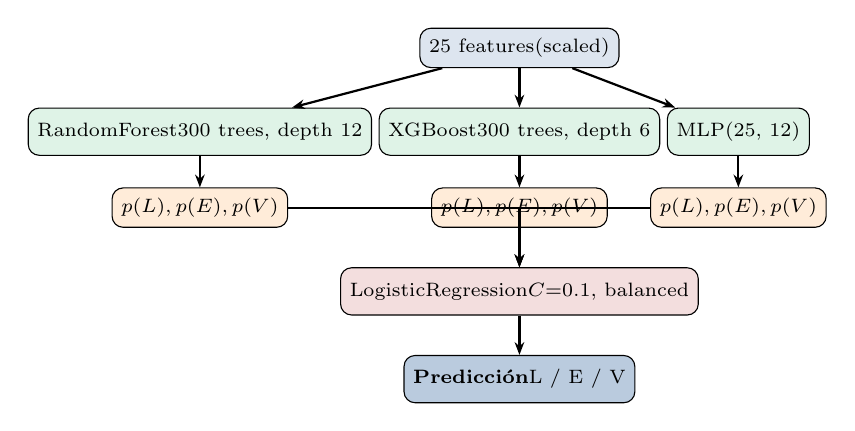
\begin{tikzpicture}[
      font=\scriptsize,
      feat/.style={draw, rounded corners, fill=azul!15,
                   minimum width=1.8cm, minimum height=0.5cm},
      model/.style={draw, rounded corners, fill=verde!15,
                    minimum width=1.6cm, minimum height=0.6cm},
      probs/.style={draw, rounded corners, fill=orange!15,
                    minimum width=1.2cm, minimum height=0.5cm},
      meta/.style={draw, rounded corners, fill=rojo!15,
                   minimum width=1.8cm, minimum height=0.6cm},
      arrow/.style={-{Stealth[scale=0.7]}, thick} ]

    \node[feat] (feat) {25 features\\ (scaled)};

    \node[model, below left=0.5cm and 0.6cm of feat] (rf)
      {RandomForest\\ 300 trees, depth 12};
    \node[model, below=0.5cm of feat] (xgb)
      {XGBoost\\ 300 trees, depth 6};
    \node[model, below right=0.5cm and 0.6cm of feat] (mlp)
      {MLP\\ (25, 12)};

    \node[probs, below=0.4cm of rf] (prf) {$p(L), p(E), p(V)$};
    \node[probs, below=0.4cm of xgb] (pxgb) {$p(L), p(E), p(V)$};
    \node[probs, below=0.4cm of mlp] (pmlp) {$p(L), p(E), p(V)$};

    \node[meta, below=0.5cm of pxgb] (meta) {LogisticRegression\\ $C{=}0.1$, balanced};

    \node[draw, rounded corners, fill=azul!30,
          minimum width=2cm, minimum height=0.6cm,
          below=0.5cm of meta] (pred) {\textbf{Predicci\'on}\\ L / E / V};

    \draw[arrow] (feat) -- (rf);   \draw[arrow] (rf)  -- (prf);
    \draw[arrow] (feat) -- (xgb);  \draw[arrow] (xgb) -- (pxgb);
    \draw[arrow] (feat) -- (mlp);  \draw[arrow] (mlp) -- (pmlp);
    \draw[arrow] (prf)  -| (meta);
    \draw[arrow] (pxgb) -- (meta);
    \draw[arrow] (pmlp) -| (meta);
    \draw[arrow] (meta) -- (pred);
  \end{tikzpicture}
\end{frame}

% ══════════════════════════════════════════════════════════════════
\begin{frame}{Entrenamiento y validaci\'on temporal}
  \textbf{Estrategia:} split temporal 80/20 --- \alert{sin leakage}

  \[
  \underbrace{2018\text{--}2024}_{\text{80\% train}} \quad
  \underbrace{2024\text{--}2026}_{\text{20\% test}}
  \]

  \vspace{0.3cm}
  \begin{columns}[T]
    \begin{column}{0.48\textwidth}
      \textbf{Balance de clases:}
      \begin{itemize}\small
        \item \code{class\_weight='balanced'} en RF y meta-LR
        \item \code{sample\_weight} en XGBoost
        \item Empates predichos: $\sim$27\% (real: 23.2\%)
      \end{itemize}
    \end{column}
    \begin{column}{0.48\textwidth}
      \textbf{Reentrenamiento final:}
      \begin{itemize}\small
        \item Validaci\'on sobre $\sim$1\,640 partidos
        \item Retrain en \textbf{todos} los datos (8\,204)
        \item Predicci\'on con modelo final
      \end{itemize}
    \end{column}
  \end{columns}
\end{frame}

% ══════════════════════════════════════════════════════════════════
\begin{frame}{Rendimiento en validaci\'on temporal}
  \centering
  \begin{tabular}{lcc}
    \toprule
    \textbf{M\'etrica} & \textbf{Valor} & \textbf{Benchmark} \\
    \midrule
    Accuracy            & \pct{61.89} & 33\% (azar) \\
    Log-loss            & 0.8185      & 1.099 (azar) \\
    F1 macro            & 0.5911      & --- \\
    MCC                 & 0.4147      & 0 (azar) \\
    Top-2 accuracy      & $\sim$87\% & --- \\
    ECE (calibraci\'on) & 0.0254      & 0 (perfecto) \\
    \bottomrule
  \end{tabular}

  \vspace{0.3cm}
  {\small
  \textbf{Per-modelo (base accuracy):}
  \[
  \text{RF } 63.0\% \quad
  \text{XGB } 62.5\% \quad
  \text{MLP } 64.8\% \quad
  \textbf{Stacking } 61.9\%
  \]
  El stacking mejora calibraci\'on y F1, no necesariamente accuracy.
  }
\end{frame}

% ══════════════════════════════════════════════════════════════════
\begin{frame}{Dixon-Coles: Predicci\'on de scores exactos}
  \textbf{Motivaci\'on:} Poisson simple subestima empates 0-0 y 1-1.\\[0.3cm]

  \textbf{Soluci\'on:} correcci\'on $\tau$ (Dixon \& Coles, 1997):

  \[
  P(X{=}x, Y{=}y) = \tau_{\rho}(x,y)\;
  \frac{e^{-\lambda}\lambda^x}{x!}\;
  \frac{e^{-\mu}\mu^y}{y!}
  \]

  con $\rho = -0.13$ y correcciones para $(0,0),(1,0),(0,1),(1,1)$.\\[0.3cm]

  \textbf{Proceso:}
  \begin{enumerate}\small
    \item Calcular $\lambda,\mu$ desde ELO:
          $\displaystyle\frac{\lambda}{\mu} = 10^{\Delta\text{ELO}/400}$
    \item Construir matriz $11\times11$ con PMF anal\'itica
    \item Aplicar $\tau$ y renormalizar
    \item Monte Carlo: 50\,000 muestras $\to$ ranking de scores
  \end{enumerate}
\end{frame}

% ══════════════════════════════════════════════════════════════════
\begin{frame}{Resultados: Octavos de Final (16avos)}
  \centering
  {\small
  \begin{tabular}{lccclc}
    \toprule
    \textbf{Partido} & \textbf{TR} & \textbf{SC} & \textbf{AV} \\
    \midrule
    Germany vs Paraguay   & \xmark & \xmark & \xmark \\
    France vs Sweden      & \cmark & \xmark & \cmark \\
    South Africa vs Canada & \cmark & \xmark & \cmark \\
    Netherlands vs Morocco & \xmark & \xmark & \xmark \\
    Portugal vs Croatia   & \cmark & \xmark & \cmark \\
    Spain vs Austria      & \cmark & \xmark & \cmark \\
    US vs Bosnia          & \cmark & \xmark & \cmark \\
    Belgium vs Senegal    & \xmark & \xmark & \xmark \\
    Brazil vs Japan       & \cmark & \xmark & \cmark \\
    Ivory Coast vs Norway & \cmark & \xmark & \cmark \\
    Mexico vs Ecuador     & \xmark & \xmark & \xmark \\
    England vs Congo DR   & \cmark & \xmark & \cmark \\
    Argentina vs Cape Verde & \cmark & \xmark & \cmark \\
    Australia vs Egypt    & \xmark & \cmark & --- \\
    Switzerland vs Algeria & \cmark & \xmark & \cmark \\
    Colombia vs Ghana     & \cmark & \xmark & \cmark \\
    \midrule
    \textbf{Total} & \pct{69} & \pct{6} & \pct{73} \\
    \bottomrule
  \end{tabular}
  }
\end{frame}

% ══════════════════════════════════════════════════════════════════
\begin{frame}{Resultados: Cuartos de Final (8avos)}
  \centering
  {\small
  \begin{tabular}{lccclc}
    \toprule
    \textbf{Partido} & \textbf{TR} & \textbf{SC} & \textbf{AV} \\
    \midrule
    Paraguay vs France    & \cmark & \xmark & \cmark \\
    Canada vs Morocco     & \cmark & \xmark & \cmark \\
    Portugal vs Spain     & \cmark & \xmark & \cmark \\
    US vs Belgium         & \cmark & \xmark & \cmark \\
    Brazil vs Norway      & \xmark & \xmark & \xmark \\
    Mexico vs England     & \xmark & \xmark & \cmark \\
    Argentina vs Egypt    & \cmark & \xmark & \cmark \\
    Switzerland vs Colombia & \xmark & \xmark & \xmark \\
    \midrule
    \textbf{Total} & \pct{62} & \pct{0} & \pct{75} \\
    \bottomrule
  \end{tabular}
  }

  \vspace{0.4cm}
  {\small
  \textbf{Partidos cr\'iticos fallados:}
  \begin{itemize}
    \item Brazil vs Norway: modelo daba Empate 49\% $\to$ Norway gan\'o 1-2
    \item Switzerland vs Colombia: Colombia favorito 69\% $\to$ Suiza avanz\'o en penales
  \end{itemize}
  }
\end{frame}

% ══════════════════════════════════════════════════════════════════
\begin{frame}{Pron\'ostico: Semifinales (4tos)}
  \centering
  {\small
  \begin{tabular}{lcccc}
    \toprule
    \textbf{Partido} & \textbf{Local} & \textbf{Empate} & \textbf{Visitante} & \textbf{Score ML} \\
    \midrule
    France   vs Morocco   & \pct{50.0} & \pct{38.9} & \pct{11.0} & 2-0 (13.9\%) \\
    Spain    vs Belgium   & \pct{61.0} & \pct{31.2} & \pct{7.8}  & 2-0 (16.8\%) \\
    Norway   vs England   & \pct{13.8} & \pct{43.4} & \pct{42.8} & 1-1 (13.3\%) \\
    Argentina vs Swiss    & \pct{50.7} & \pct{39.0} & \pct{10.3} & 2-0 (14.3\%) \\
    \bottomrule
  \end{tabular}
  }

  \vspace{0.3cm}
  {\small
  \begin{tabular}{lcc}
    \toprule
    \textbf{Partido} & \textbf{$\lambda$ local} & \textbf{$\lambda$ visit.} \\
    \midrule
    France   vs Morocco   & 2.06 & 0.67 \\
    Spain    vs Belgium   & 2.29 & 0.44 \\
    Norway   vs England   & 1.22 & 1.51 \\
    Argentina vs Swiss    & 2.09 & 0.64 \\
    \bottomrule
  \end{tabular}
  }

  \vspace{0.3cm}
  Partidos a jugarse el 9--11 de julio de 2026.
\end{frame}

% ══════════════════════════════════════════════════════════════════
\begin{frame}{Tracker en vivo: bracket\_tracker.py}
  \textbf{M\'etricas duales por partido:}

  \vspace{0.2cm}
  \begin{tabular}{lll}
    \toprule
    \textbf{M\'etrica} & \textbf{Mide} & \textbf{Ejemplo} \\
    \midrule
    T.Regular (TR) & Ganador en 90' (L/E/V) & Alemania 64\% $\to$ Empate \xmark \\
    Marcador (SC)  & Score exacto            & 1-1 $\to$ 1-1 \cmark \\
    Clasificaci\'on (AV) & Avance (incl. penales) & Alemania 77\% $\to$ Paraguay \xmark \\
    \bottomrule
  \end{tabular}

  \vspace{0.4cm}
  \textbf{Funcionalidades:}
  \begin{itemize}\small
    \item Tabla textual + 4 gr\'aficas profesionales
    \item Fallback JSON cuando results.csv no tiene el partido
    \item Auto-detecci\'on de avance si hay ganador claro en 90'
    \item Soporta \code{--8avos}, \code{--4tos}, \code{--graphs}, \code{--save}
  \end{itemize}
\end{frame}

% ══════════════════════════════════════════════════════════════════
\begin{frame}{Visualizaciones}
  \begin{columns}[T]
    \begin{column}{0.33\textwidth}
      \centering
      \includegraphics[width=\textwidth]{data/4tos_advancement.png}\\
      {\small Avance a Semifinales}
    \end{column}
    \begin{column}{0.33\textwidth}
      \centering
      \includegraphics[width=\textwidth]{data/4tos_confidence.png}\\
      {\small Confianza del modelo}
    \end{column}
    \begin{column}{0.33\textwidth}
      \centering
      \includegraphics[width=\textwidth]{data/4tos_poisson_scores.png}\\
      {\small Dixon-Coles scores}
    \end{column}
  \end{columns}
  \vspace{0.3cm}
  {\small
  \centering
  4 gr\'aficas por ronda: avance, probabilidades, confianza y scores.
  Generadas con \code{show\_results.py --4tos --save}.
  }
\end{frame}

% ══════════════════════════════════════════════════════════════════
\begin{frame}{Stacking: Bracket Overview}
  \centering
  \includegraphics[width=0.8\textwidth]{data/4tos_bracket_overview.png}\\
  {\small Pizarra de resultados: cards con TR/SC/AV por partido}
\end{frame}

% ══════════════════════════════════════════════════════════════════
\begin{frame}{Resumen y conclusiones}
  \begin{itemize}
    \item \textbf{Modelo:} stacking ensemble
      (RF + XGB + MLP $\to$ LR) con 25 features
    \item \textbf{Validaci\'on:} split temporal 80/20,
      \pct{61.89} accuracy, F1 macro 0.59, MCC 0.41
    \item \textbf{Resultados 16avos:} \pct{69} TR, \pct{73} AV
    \item \textbf{Resultados 8avos:} \pct{62} TR, \pct{75} AV
    \item \textbf{Pr\'oximo:} 4 partidos de Semifinales (9--11 jul)
  \end{itemize}

  \vspace{0.5cm}
  \textbf{Mejoras futuras:}
  \begin{itemize}\small
    \item NLP features con datos hist\'oricos
    \item Calibraci\'on Platt del meta-modelo
    \item Incorporar datos de alineaciones/lesiones
  \end{itemize}

  \vspace{0.5cm}
  \centering
  \code{github.com:elable947/predWC.git}
\end{frame}

\end{document}
